\section{Adafruit Bonnet}

All inputs and outputs are managed through the Adafruit 1.3" Color TFT Bonnet for Raspberry Pi \cite{adafruitwebsite}. This bonnet includes a 240x240 pixel TFT display, a joystick, and two buttons. The button inputs are read through a standard GPIO interface, while the display is driven by the ST7789V chip connected via SPI.

To integrate the Adafruit Bonnet, an example program (\texttt{example\_adafruit\_bonnet}) \cite{projectRepo} was created to test its functionality and ensure compatibility with the board. This program will potentially be integrated into the X-HEEP GitHub repository for future projects involving input/output operations with the Adafruit bonnet.

\begin{figure}[ht]
    \centering
    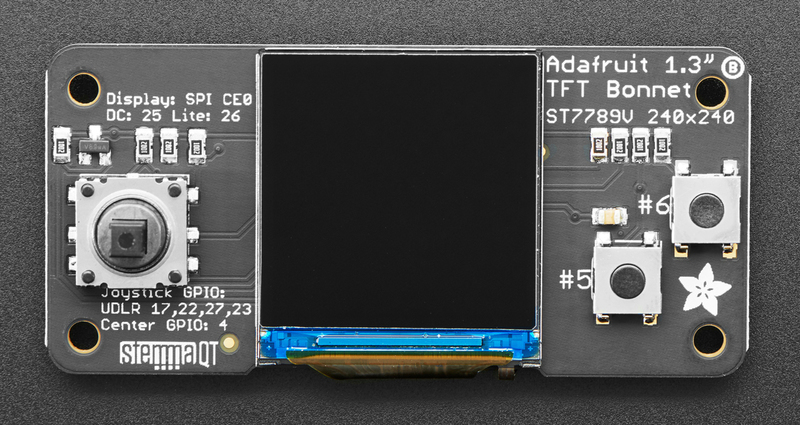
\includegraphics[width=0.6\textwidth]{images/Adafruit_Front.jpg}
    \caption{Adafruit 1.3" Color TFT Bonnet for Raspberry Pi \cite{adafruitwebsite}}
    \label{fig:adafruitFront}
\end{figure}


\subsection{Buttons}


There are six buttons in total: a joystick on the left side of the display (UP, DOWN, LEFT, and RIGHT), and two buttons (A and B) on the right side of the display.
They need to be initialized once and then read once at every loop in the game. The \texttt{example\_adafruit\_bonnet} implements them by reading the logic value of the six pins and filling in 3 arrays to determine their current state and if they are at positive or negative edge by comparing with their last state. Reading the buttons by polling aligns with DOOM's input handling. There is no hardware interrupt in DOOM.

Implementing button functionality was facilitated by the existing \texttt{example\_gpio\_intr} application from the x-heep repository \cite{xHeepRepo}. \\


\subsection{Display Driver Development}

The display module works by receiving an initializaiton sequence once after power on and then receiving information about the pictures to draw. To draw a picture it first requires to receive the X and Y coordinates of the pixels in the upper left and lower right corners of a rectangle and then the color of every pixel row-wise. This permits the user to chose, what portion of the display needs to be drawn. DOOM operates by rendering graphics to a screen buffer, which is then displayed on the screen. Therefore Doom redraws the whole display every time.

The integration of the Adafruit Bonnet's display proved more complex than expected. Originally designed for Raspberry Pi with a Python-based driver, the display uses the ST7789 chip, common in TFT displays. Several existing driver implementations exist for the ST7789 chip, including the Arduino ST7789 Fast library on GitHub \cite{arduinoST7789}, which served as a reference for this project.

\subsubsection*{Communication with the Display}

The ST7789 communicates with the board via an SPI interface, utilizing the MOSI (Master Out Slave In), SCK (Serial Clock), and CS (Chip Select) pins. Notably, the ST7789 also requires a DC (Data/Command) line to distinguish between data and command transmissions, which poses a challenge on X-HEEP's implementations on FPGA and HEEPocrates: \\

In the X-HEEP implementation on the PYNQ-Z2 FPGA, the SPI interface is pre-implemented. It consists of the four standard signals MOSI, MISO (Master In Slave Out), SCK, and CS.  However, the FPGA cannot directly control the DC signal through SPI. Thus the DC pin's behaviour needs to be manually emulated on a GPIO pin. \\
Initially, this didn't work and the display stayed black. After some experimentation with an Arduino, the problem was diagnosed to be the initialization sequence of the display. When the display was powered on, received the initialization sequence by pluging it into the Arduino and then switching the SPI cables to the FPGA, it was possible to display an image from the FPGA. A logic analyzer was used to debug the problem (see Figure \ref{fig:Logic_analyzer_zoom_in}). \\
In the end the problem turned out to be the DC pin: \\
When X-HEEP gives a command to the SPI module, it will execute it once the module is ready. The GPIO function, however, is instant. As a consequence, it can happen that the FPGA is sending a command, while the DC pin already signals, that it is sending data. Adding a delay between different initialization commands resolved the issue. Performance wise this is not a problem, as the initialization sequence is only played once.

This issue significantly delayed the project, compounded by an initial display unit with a bad contact on the display ribbon cable.

\begin{figure}[ht]
    \centering
    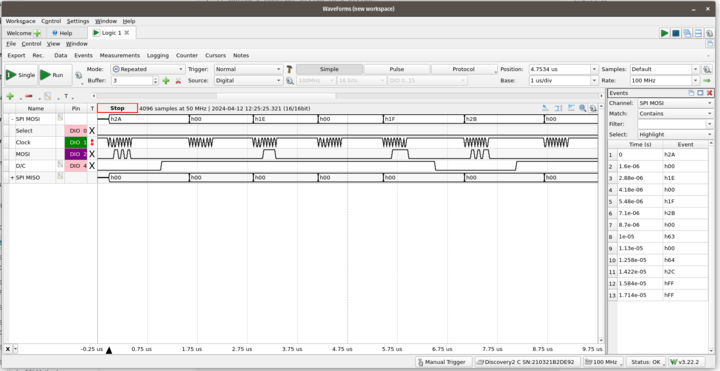
\includegraphics[width=0.8\textwidth]{images/Logic_analyzer_zoom_in.png}
    \caption{Detailed view of the correct display initialization sequence on a logic analyzer.} 
    \label{fig:Logic_analyzer_zoom_in}
\end{figure}

With the issues resolved, a new device BSP driver library (\texttt{sw/device/bsp/ST7789}) \cite{projectRepo} has been created for the ST7789 chip. During the creation of that library, other issues arose. Copying functions from the test file to the library, suddenly made them perform differently. The initialization sequence still worked fine. This time, however, it was the image transmission that didn't work anymore. After some troubleshooting it was found out that the problem was again linked to the DC pin, which is not synched with the SPI signal. The initialization signal had no issue as there were already delays between the signals. To send an image, however, the device also starts by sending the start and end pixel of the rectangle to fill in as a command. Then it sends the color information for each pixel as data. It is unclear why this problem only arose when the functions were moved into the bsp library. The issue was solved by adding a delay to all functions that switch between command and data. Performance wist this doesn't affec performance greatly, as the bulk transfer of pixels doesn't need delays, as there is no switching between data and commands. The working bsp library will probably be added to the main X-HEEP repository.

The example program \texttt{example\_adafruit\_bonnet} shows the working of buttons and display by showing a 120x120 pixels image of the ESL Logo. When a button is pressed, the picture moves by two pixels in the direction of the pressed button and a message is sent on the UART terminal for each positive and negative edge of a button.

\newpage

\subsection{Pinout Configuration}

On the PYNQ-Z2 FPGA, the buttons are connected to the following pins:

\begin{table}[!ht]
    \centering
    \begin{tabular}{|c|c|c|c|}
        \hline
        \textbf{Description} & \textbf{PYNQ-Z2 PIN} & \textbf{Physical Location} & \textbf{Software PIN} \\
        \hline
        \hline
        Joystick UP & U8 & Raspberry Pi 15 & GPIO 9 \\
        \hline
        Joystick DOWN & V7 & Raspberry Pi 13 & GPIO 10 \\
        \hline
        Joystick LEFT & U7 & Raspberry Pi 11 & GPIO 11 \\
        \hline
        Joystick RIGHT & V6 & Raspberry Pi 8 & GPIO 12 \\
        \hline
        Button A & U13 & Arduino AR2 & GPIO 13 \\
        \hline
        Button B & V13 & Arduino AR3 & GPIO 14 \\
        \hline
        \hline
        Display CLK & H15 & Arduino SPI 3 & spi\_sck\_o \\
        \hline
        Display MOSI & T12 & Arduino SPI 4 & spi\_sd\_io[0] \\
        \hline
        Display CS & F16 & Arduino SPI 5 & spi\_csb\_o \\
        \hline
        Display DC & V8 & Raspberry Pi 19 & GPIO 8 \\
        \hline
    \end{tabular}
    \caption{Overview of the connections between the PYNQ-Z2 FPGA and the Adafruit Bonnet}
    \label{table:pinout_Adafruit}
\end{table}

\begin{figure}[!ht]
    \centering
    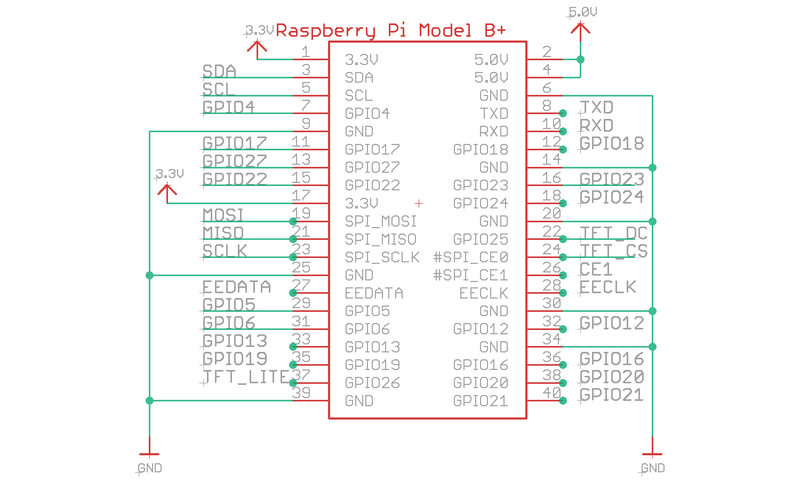
\includegraphics[width=\textwidth]{images/adafruit_PINOUT.png}
    \caption{Adafruit Bonnet PINOUT diagram \cite{adafruitwebsite}}
    \label{fig:adafruitPinout}
\end{figure}

\begin{figure}[!ht]
    \centering
    \rotatebox{90}{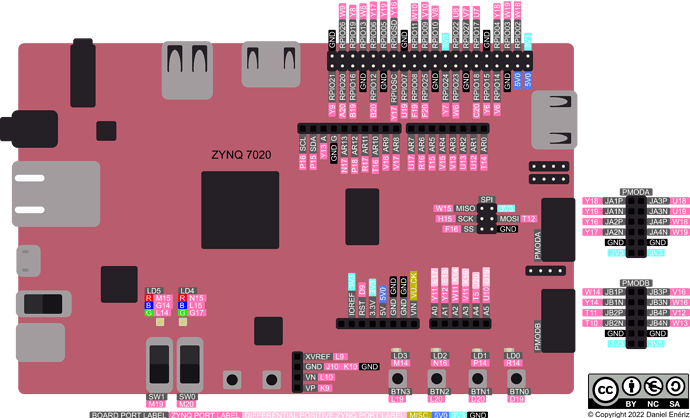
\includegraphics[width=1.5\textwidth]{images/PYNQ-Z2_PINOUT.png}}
    \caption{Pinout of PYNQ-Z2 FPGA \cite{pynqPinout}}
    \label{fig:pynqPINOUT}
\end{figure}


